\documentclass{article}
% Author: Luan Leal
% Last update: 2024-12-03

% ----------------------------

% ----------------------------   IMPORTS   ----------------------------
\usepackage{amssymb, amsthm, amsmath, geometry, siunitx, caption, float, graphicx}
\usepackage{enumitem}
\usepackage[utf8]{inputenc}
\usepackage[onehalfspacing]{setspaceenhanced}
\usepackage[brazil]{babel} % Adaptação ao pt-br
\usepackage{hyperref} % Usado para inserir links
\usepackage[capitalize, brazilian, noabbrev]{cleveref} % Referência adaptada ao pt-br
\usepackage{subcaption}
\usepackage{makecell}
\usepackage[num,overcite]{abntex2cite}

% ----------------------------   LAYOUT   ----------------------------
\citebrackets[]
\geometry{a4paper, lmargin=3cm, tmargin=3cm, rmargin=2cm, bmargin=2cm}
\onehalfspacing
%\setlength{\parindent}{45pt}
\sisetup{output-decimal-marker = {,}}

% ----------------------------  THEOREMS  ----------------------------
% -Ambiente de definição
\theoremstyle{definition}
\newtheorem{dfn}{Definição}[section]

% -Ambiente de observação
\theoremstyle{remark}
\newtheorem{obs}{Observação}

% -Ambiente de lema
\theoremstyle{definition}
\newtheorem{lema}{Lema}

% -Ambiente de exemplo
\theoremstyle{definition}
\newtheorem{xp}{Exemplo}[section]

% -Ambiente de proposição
\newtheorem{prop}{Proposição}

% -Ambiente de teorema e demonstração
\theoremstyle{plain}
\newtheorem{thm}{Teorema}
\theoremstyle{remark}
\newtheorem*{dms}{Demonstração}

% -Ambiente de exercício e resolução
\theoremstyle{definition}
\newtheorem{xcs}{Exercício}
\theoremstyle{remark}
\newtheorem*{rsl}{Resolução}

% ----------------------------  COMMANDS  ----------------------------
%\newcommand{\RR}{\mathbb{R}} % \mathbb{R} = \RR
%\newcommand{\ZZ}{\mathbb{Z}} % \mathbb{Z} = \ZZ

\newcommand{\commentspace}{\\ \textbf{Espaço para comentários:} \vspace{10\baselineskip}}
\DeclareSIUnit{\calorie}{cal}
\author{Luan Leal (15470820); Matheus Justino (14598021);\\ 
Matheus Queiroz (15479562); Micael Baruch (15578823)}
\title{Prova 3 --- Química II}

\begin{document}
\maketitle

    \textbf{(1)} O fluoreto de nitrila (\ce{NO2F}) é um gás incolor e um agente oxidante forte empregado como agente fluoretante. É uma espécie molecular (não iônica) e possui estrutura planar. O estudo de suas propriedades termodinâmicas e de sua formação foi realizado em 1962 por E. Tschuikow-Row\textsuperscript{1}, o qual verificou o mecanismo de formação e sua dependência com a temperatura através de espectroscopias vibracionais (Raman e IV).\\

A reação global observada foi:
\begin{align*}
    2\,\ce{NO2}(g) + \ce{F2}(g) \rightarrow 2\,\ce{NO2F}(g)
\end{align*}

 Essa reação, no entanto, apresentou um mecanismo complexo cuja lei de velocidade é dada por:
\begin{align*}
    v = k[\ce{NO2}][\ce{F2}]
\end{align*}

e o estudo de suas propriedades termodinâmicas apresentou variação da constante de equilíbrio ($K_{\text{eq}}$) em função da temperatura na etapa determinante (etapa lenta), conforme (ln$K_{\text{eq}}$) na tabela abaixo:

\begin{center}
\begin{tabular}{|c|c|c|c|c|c|c|c|c|c|}
\hline
\textbf{T / K} & 200 & 300 & 400 & 500 & 600 & 700 & 800 & 900 & 1000 \\
\hline
\textbf{ln $K_{\text{eq}}$} & 7,55 & 14,43 & 17,84 & 19,85 & 21,16 & 22,08 & 22,72 & 23,28 & 23,67 \\
\hline
\end{tabular}
\end{center}

\bigskip

Com todas essas informações em mãos:\\

\textbf{a)} Proponha o mecanismo de reação para a formação do \ce{NO2F} e explicite a etapa determinante;\\

\textbf{Resposta:} 

Para propor o mecanismo de reação para a formação do \ce{NO2F}, partimos da equação global observada:
\begin{align*}
2\ \ce{NO2}(g) + \ce{F2}(g) \rightarrow 2\ \ce{NO2F}(g)
\end{align*}

Embora a reação pareça simples, estudos experimentais revelaram que ela ocorre por um mecanismo mais complexo, sendo a sua velocidade regida pela expressão:
\begin{align*}
v = k[\ce{NO2}][\ce{F2}]
\end{align*}

Essa lei de velocidade indica que a etapa determinante (ou etapa lenta) do processo envolve uma colisão entre uma molécula de \ce{NO2} e uma molécula de \ce{F2}, ou seja, é uma etapa bimolecular. A partir disso, propõe-se o seguinte mecanismo:

\textit{Etapa lenta (determinante):}
\begin{align*}
\ce{NO2 + F2 -> NO2F + F}
\end{align*}

\textit{Etapa rápida:}
\begin{align*}
\ce{F + NO2 -> NO2F}
\end{align*}

Somando as etapas:
\begin{align*}
&\ce{NO2 + F2 -> NO2F + F} \hspace{1.0cm} \text{(etapa lenta)}\\
&\ce{F + NO2 -> NO2F} \hspace{1.8cm} \text{(etapa rápida)}\\
\midrule %Alguém sabe ajeitar essa linha maldita?
&\ce{2NO2 + F2 -> 2NO2F} \hspace{1.2cm} \text{(equação global)}
\end{align*}

Dessa forma, o mecanismo é consistente tanto com a estequiometria global quanto com a lei de velocidade observada experimentalmente, e evidencia que a etapa determinante é a formação do intermediário a partir de \ce{NO2} e \ce{F2}.

\vspace{0.4cm}

\textbf{b)} Proponha a estrutura do complexo ativado para essa reação bimolecular;\\

\textbf{Resposta:} 

Para representar a estrutura do complexo ativado dessa reação bimolecular, é necessário considerar que, durante a colisão entre \ce{NO2} e \ce{F2}, ocorre uma reorganização eletrônica na qual uma das ligações F–F começa a se romper ao mesmo tempo que uma nova ligação N–F começa a se formar. Esse estado de transição pode ser representado por uma estrutura em que os átomos ainda não estão completamente ligados, caracterizando o chamado “complexo ativado” ou “estado de transição”.

A estrutura pode ser descrita como:
\begin{align*}
\ce{[NO2 \cdots F \cdots F]^{\ddagger}}
\end{align*}

Nesse intermediário, o flúor mais próximo do nitrogênio do \ce{NO2} apresenta uma ligação parcialmente formada com o N, enquanto a ligação F–F encontra-se parcialmente rompida. Além disso, a geometria ao redor do nitrogênio provavelmente se torna levemente distorcida em relação ao plano original da molécula, dada a reorganização eletrônica em curso. Essa estrutura representa o ponto de maior energia no caminho da reação, ou seja, o topo da barreira energética que os reagentes devem superar para formar os produtos.

\vspace{0.4cm}

\textbf{c)} Apresente a curva de energia potencial de formação do \ce{NO2F}, apontando a região da curva onde ocorre a formação do complexo ativado. De acordo com suas observações, essa reação é endotérmica ou exotérmica? Explique com o devido formalismo.\\

\textbf{Resposta:} 

Com base nos dados fornecidos sobre a constante de equilíbrio (\(K_\text{eq}\)) da etapa determinante em diferentes temperaturas, é possível analisar a natureza energética do processo e determinar se a reação é endotérmica ou exotérmica. A tabela mostra que o valor de \(\ln(K_\text{eq})\) aumenta com o aumento da temperatura, o que implica que a constante de equilíbrio também cresce. Isso pode ser interpretado por meio da equação de Van’t Hoff:
\begin{align*}
\ln(K_\text{eq}) = -\frac{\Delta H^\circ}{R} \cdot \frac{1}{T} + \frac{\Delta S^\circ}{R}
\end{align*}

Esta equação lineariza a relação entre \(\ln(K_\text{eq})\) e o inverso da temperatura \(1/T\). Uma análise preliminar da tabela de dados já indicava que o valor de \(\ln(K_\text{eq})\) aumenta com o aumento da temperatura. Esse comportamento é característico de reações endotérmicas, pois o equilíbrio se desloca para a direita (formação de produtos) com o aumento da temperatura, o que implica um \(\Delta H^\circ\) positivo.

Para quantificar essa variação de entalpia, realizamos uma regressão linear dos dados de \(\ln(K_\text{eq})\) em função de \(1/T\). O gráfico resultante dessa regressão está apresentado na (\cref{fig:vant})

\begin{figure}[H]
\centering
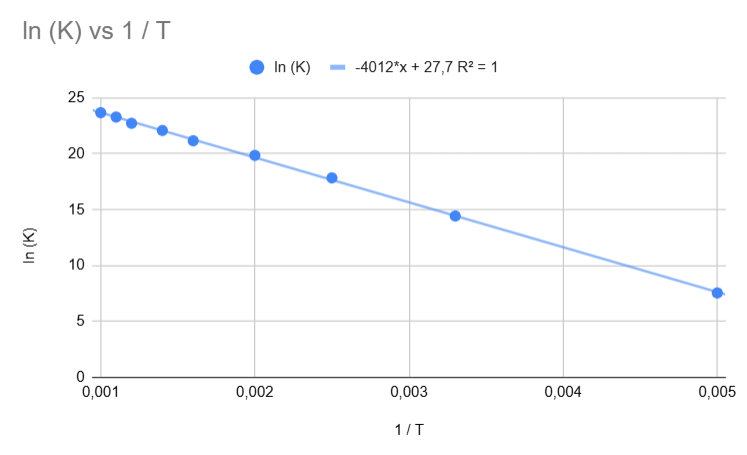
\includegraphics[width=0.7\linewidth]{fig/regressao.png}
\caption{Gráfico de \(\ln(K_\text{eq})\) versus \(1/T\) para a etapa determinante, com a linha de regressão linear.}
\label{fig:vant}
\end{figure}

A partir da regressão linear, obtivemos a equação da reta que descreve o comportamento dos dados:
\begin{align*}
\ln(K_\text{eq}) = -4012 \text{ K} + 27,7
\end{align*}

Comparando esta equação com a forma linear da Equação de Van't Hoff \(y = mx + b\), identifica-se diretamente o coeficiente angular da reta como \(m = -4012 \text{ K}\). Pela Equação de Van't Hoff, sabemos que o coeficiente angular é \(m = -\frac{\Delta H^\circ}{R}\). Portanto, podemos rearranjar a equação para calcular \(\Delta H^\circ\):
\begin{align*}
    \Delta H^\circ = -m \times R
\end{align*}

Substituindo os valores conhecidos do coeficiente angular e da constante dos gases ideal \(R = 8.314 \frac{J}{mol.K}\):
\begin{align*}
& \Delta H^\circ = -(-4012 \text{ K}) \times (8.314 \text{ J} \cdot \text{mol}^{-1} \cdot \text{K}^{-1}) \\
& \Delta H^\circ = 4012 \times 8.314 \text{ J} \cdot \text{mol}^{-1} \\
& \Delta H^\circ = 33355.768 \text{ J} \cdot \text{mol}^{-1}
\end{align*}

Convertendo o valor para quilojoules por mol \(kJ/mol\), para maior clareza e padronização em termodinâmica:
\begin{align*}
    \Delta H^\circ \approx +33.35 \text{ kJ} \cdot \text{mol}^{-1}
\end{align*}

O resultado obtido, $\Delta H^\circ = +33.35 \text{ kJ} \cdot \text{mol}^{-1}$, indica que a variação de entalpia para a etapa determinante da reação de formação do $\ce{NO2F}$ é positiva, ou seja, que a etapa determinante da reação de formação do $\ce{NO2F}$ é endotérmica. Isso significa que essa etapa absorve energia do ambiente para prosseguir.

Essa característica endotérmica é ilustrada no diagrama de energia potencial em função da coordenada de reação (\cref{diagrama}). No diagrama, os reagentes se encontram em um patamar energético inicial. À medida que a reação prossegue, a energia do sistema aumenta até atingir um máximo, correspondente ao complexo ativado — o ponto mais instável e de maior energia do processo. Após ultrapassada essa barreira, a energia diminui com a formação dos produtos.

    \begin{figure}[H]
        \centering
        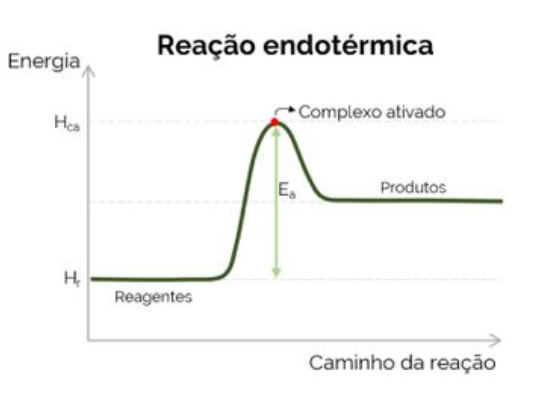
\includegraphics[width=0.35\linewidth]{fig/grafico.png}
        \caption{curva de energia potencial de formação do \ce{NO2F}}
        \label{diagrama}
    \end{figure}

Como a energia dos produtos é maior do que a dos reagentes, a variação de entalpia total da reação (\(\Delta H\)) é positiva, reforçando que o processo é endotérmico. A energia de ativação (\(E_\text{a}\)) corresponde à diferença entre os reagentes e o complexo ativado, e sua magnitude está relacionada à taxa com que a reação ocorre: quanto maior a \(E_\text{a}\), mais lenta é a reação, justificando a sua presença como etapa determinante.

Portanto, a partir da análise dos dados de equilíbrio via regressão linear pela Equação de Van't Hoff e da representação no diagrama de energia, conclui-se que a formação do \ce{NO2F} apresenta uma etapa lenta que é endotérmica, com formação de um complexo ativado de alta energia, e que a reação global ocorre mediante superação dessa barreira, em consonância com o modelo energético das reações químicas e o formalismo termodinâmico.


    \textbf{(2)} Considere que a decomposição térmica do \ce{N2O5} gasoso segue o seguinte mecanismo:
\begin{align*}
    \ce{N2O5 &->[{k_1}] NO2 + NO3}\\
    \ce{NO2 + NO3 &->[{k_{-1}}] N2O5}\\
    \ce{NO2 + NO3 &->[{k_2}] NO2 + O2 + NO}\\
    \ce{NO + N2O5 &->[{k_3}] 3NO2}
\end{align*}

\textbf{a)} Usando a aproximação do estado estacionário para as espécies \ce{NO3} e \ce{NO}, obtenha a lei cinética derivada do mecanismo proposto.

\textbf{Resposta:}

A velocidade global da reação é dada pela taxa de consumo de \ce{N2O5} e se relaciona com as constantes da seguinte forma:
\begin{align}\label{eqOrig}
    v = - \frac{d[\ce{N2O5}]}{dt} = K_1 [\ce{N2O5}] - K_{-1} [\ce{NO2}][\ce{NO3}] + K_3 [\ce{NO}][\ce{N2O5}]
\end{align}
Vamos adotar a aproximação do estado estacionário para as espécies \ce{NO3} e \ce{NO}, de forma que obtemos as seguintes equações:
\begin{align*}
    \frac{d[\ce{NO3}]}{dt} &= K_1 [\ce{N2O5}] - K_{-1} [\ce{NO2}][\ce{NO3}] - K_2 [\ce{NO2}][\ce{NO3}] \approx 0\\
    \frac{d[\ce{NO}]}{dt} &= K_2 [\ce{NO2}][\ce{NO3}] - K_3 [\ce{NO}][\ce{N2O5}] \approx 0
\end{align*}
Da primeira equação, obtemos duas relações importantes:
\begin{align*}
    [\ce{NO3}] &= \frac{K_1 [\ce{N2O5}]}{(K_{-1} + K_2) [\ce{NO2}]}\\
    K_1 [\ce{N2O5}] &= K_{-1} [\ce{NO2}][\ce{NO3}] + K_2 [\ce{NO2}][\ce{NO3}]
\end{align*}
E, da segunda equação, obtemos:
\begin{align*}
    K_2 [\ce{NO2}][\ce{NO3}] = K_3 [\ce{NO}][\ce{N2O5}]
\end{align*}
Assim, podemos substituir \( K_1 [\ce{N2O5}] \) na \cref{eqOrig}, obtendo:
\begin{align*}
    v &= 2 K_2 [\ce{NO2}][\ce{NO3}]\\
      &= 2 K_2 [\ce{NO2}] \left( \frac{K_1 [\ce{N2O5}]}{(K_{-1} + K_2) [\ce{NO2}]}  \right) \\
      &= \frac{2 K_1 K_2}{K_{-1} + K_2} [\ce{N2O5}]
\end{align*}
Sendo a expressão final a lei cinética derivada da aproximação do estado estacionário das espécies \ce{NO3} e \ce{NO}.

\textbf{b)} Obtenha a lei cinética admitindo as reações (1) e (-1) como um equilíbrio.

\textbf{Resposta:}

Assumindo equilíbrio entre as etapas (1) e (-1), obtemos:
\begin{align*}
    K_1 [\ce{N2O5}] = K_{-1} [\ce{NO2}][\ce{NO3}]
\end{align*}
Donde segue que:
\begin{align*}
    [\ce{NO3}] = \frac{K_1 [\ce{N2O5}]}{K_{-1} [\ce{NO2}]} 
\end{align*}
Agora, note que a etapa lenta deve ser a reação (2), pela premissa de equilíbrio. Além disso, note que a cada ocorrência da reação (2), temos o consumo de duas moléculas de \ce{N2O5}, uma consumida para formar os reagentes da etapa (2) e outra consumida para reagir com o \ce{NO} formado. Dessa forma, obtemos a seguinte expressão para a reação global:
\begin{align*}
    v &= 2 v_2\\
      &= 2 K_2 [\ce{NO2}][\ce{NO3}]\\
      &= \frac{2 K_1 K_2}{K_{-1}} [\ce{N2O5}]
\end{align*}
Sendo a última expressão a lei cinética.

\textbf{c)} Mostre que da lei cinética obtida em a) pode-se, através de aproximações, chegar à mesma equação obtida em b). Em que condições está justificada essa aproximação? Teste sua hipótese utilizando valores plausíveis para as constantes de velocidade (verifique na base de dados cinéticos do NIST, por exemplo).

\textbf{Resposta:}

A partir da aproximação de que \( K_{-1} >> K_2 \) obtemos que a lei cinética obtida em a) pode levar à lei cinética obtida em b), de fato, sob essa aproximação obtemos:
\begin{align*}
    \frac{2K_1K_2}{K_{-1} + K_2} [\ce{N2O5}] \approx \frac{2K_1K_2}{K_{-1}} [\ce{N2O5}] 
\end{align*}
Fisicamente, essa aproximação equivale a dizer que a velocidade com o intermediário \ce{NO3} reverte para o reagente \ce{N2O5} é muito maior que a velocidade com que ele reage para formar os produtos finais. Note que isso valida a premissa de um equilíbrio entre (1) e (-1), como esperado.

Contudo, utilizando o \textit{NIST Chemical Kinetics Database}\footnote{\url{https://kinetics.nist.gov/kinetics/Detail?id=1997DEM/SAN1-266:534}, para a etapa (-1); e \url{https://kinetics.nist.gov/kinetics/Detail?id=1997DEM/SAN1-266:532}, para a etapa (2)}, obtemos que essa aproximação não é válida, dado que, na temperatura de \qty{300}{\kelvin}, \( K_{-1} = \num{2.2e-30} \) e \( K_2 = \num{6.75e-16} \). 
%Falta isso aqui


    \textbf{(3)} Considere o sistema representado abaixo, onde um compartimento de
volume V, dividido em dois volumes de \num{0,25} V e um de \num{0,50} V. Um dos volumes
menores foi preenchido com \num{0,75} mols de \ce{N2} e o outro dos volumes menores com
\num{0,25} mols de \ce{O2}, ambos a 300 K, como ilustrado abaixo. Em um certo momento, a
barreira que divide o volume é removida.  Considere ainda que os gases são
ideais.\\

\begin{figure}[H]
    \centering
    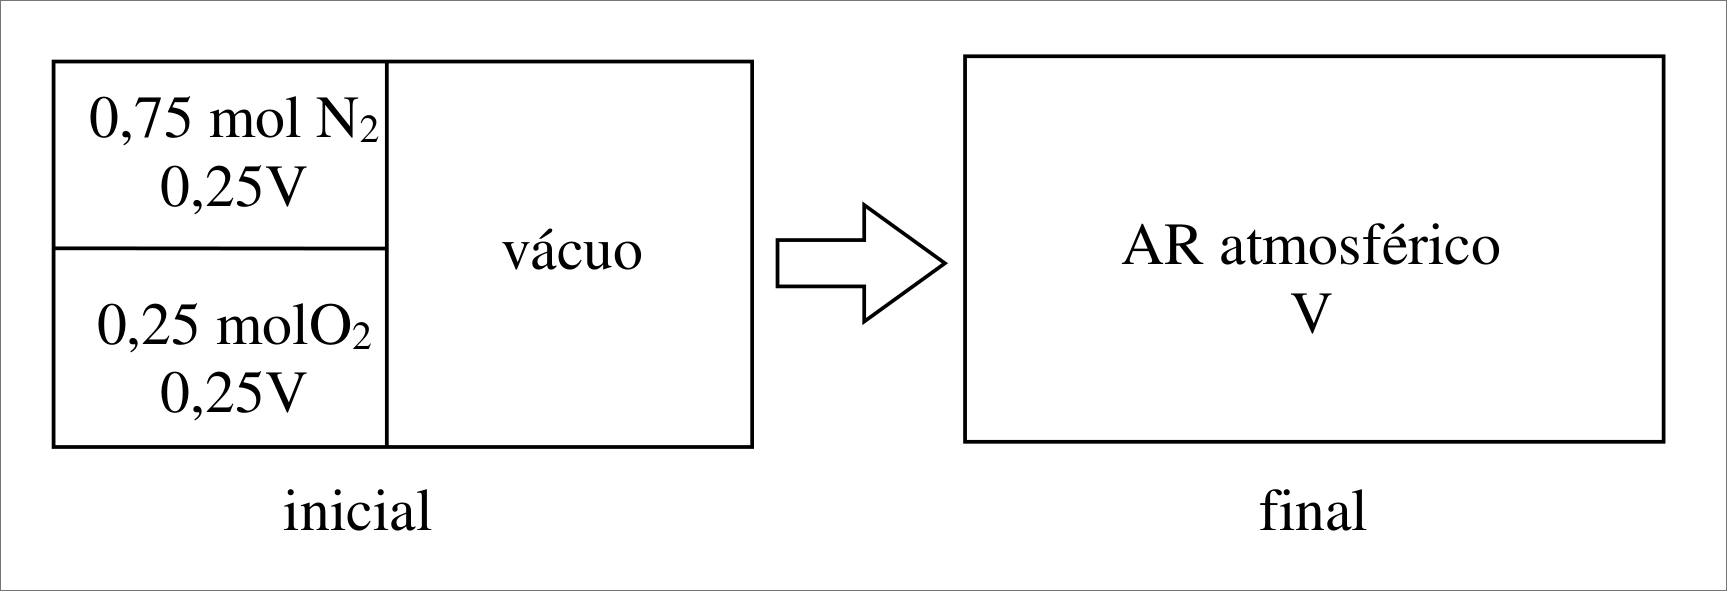
\includegraphics[width=.8\linewidth]{Q3.png}
\end{figure}

(a) Calcule a variação de entropia do \ce{N2} e do \ce{O2} entre os estados
final e inicial sabendo que a temperatura permanece constante. Indique os
cálculos a partir da derivada total apropriada.\\

    \textbf{Resposta:} Para calcular a variação de entropia de cada gás, utilizamos a expressão para a variação de entropia de um gás ideal em processo isotérmico:

    \begin{align*}
    \Delta S = nR \ln\left(\frac{V_f}{V_i}\right)
    \end{align*}
    
    Para o \ce{N2}:
    \begin{itemize}
        \item $n_{\ce{N2}} = \num{0,75}$ mol
        \item $V_i = \num{0,25}V$
        \item $V_f = V$
    \end{itemize}
    
    \begin{align*}
    \Delta S_{\ce{N2}} = \num{0,75} \cdot R \cdot \ln\left(\frac{V}{\num{0,25}V}\right) = \num{0,75}R\ln(4)
    \end{align*}

    Para o \ce{O2}:
    \begin{itemize}
        \item $n_{\ce{O2}} = \num{0,25}$ mol
        \item $V_i = \num{0,25}V$
        \item $V_f = V$
    \end{itemize}
    
    \begin{align*}
    \Delta S_{\ce{O2}} = \num{0,25} \cdot R \cdot \ln\left(\frac{V}{\num{0,25}V}\right) = \num{0,25}R\ln(4)
    \end{align*}
    
    Portanto, as variações de entropia são:
    \begin{align*}
    \boxed{\Delta S_{\ce{N2}} = \num{0,75}R\ln(4)} \quad \text{e} \quad \boxed{\Delta S_{\ce{O2}} = \num{0,25}R\ln(4)}
    \end{align*}

(b) Calcule a variação de entropia total do sistema entre o estado inicial e
final (após a remoção das divisórias).\\

    \textbf{Resposta:} A variação de entropia total do sistema é a soma das contribuições de cada gás:

    \begin{align*}
    \Delta S_{\text{total}} = \Delta S_{\ce{N2}} + \Delta S_{\ce{O2}} = \num{0,75}R\ln(4) + \num{0,25}R\ln(4) = R\ln(4)
    \end{align*}
    
    Resultando em:
    \begin{align*}
    \boxed{\Delta S_{\text{total}} = R\ln(4)}
    \end{align*}

(c) Explique porque a mistura de \ce{O2} e \ce{N2}, nas condições descritas,
pode ser considerada como um processo adiabático (\(dq= 0\)).\\

    \textbf{Resposta:} A mistura de \ce{O2} e \ce{N2} nas condições descritas pode 
    ser considerada um processo adiabático (\(dq = 0\)) porque não há transferência 
    de calor entre o sistema e a vizinhança. Isso ocorre porque a temperatura 
    permanece constante (processo isotérmico) e a expansão dos gases é irreversível, 
    sem realização de trabalho útil. Como os gases são ideais e a energia interna 
    depende apenas da temperatura, a variação de energia interna (\(\Delta U\)) é zero. 
    Pela Primeira Lei da Termodinâmica,

    \begin{align*}
    \Delta U = q + w,
    \end{align*}

    como \(\Delta U = 0\) e \(w = 0\) (não há trabalho contra uma pressão externa, 
    pois a expansão é livre no vácuo), conclui-se que \(q = 0\). Portanto, o processo 
    é adiabático. 

(d) Algumas vezes os alunos respondem o item a dizendo que a variação de
entropia é zero pois a entropia é definida como \(dS= dq_{\text{rev}}/T\) e,
sendo o processo adiabático (item c), \(dS\) também deveria ser zero. Explique
qual é o problema com esse raciocínio.\\

    \textbf{Resposta:} O raciocínio de que a variação de entropia é zero porque 
    \(dS = \frac{dq_{\text{rev}}}{T}\) e o processo é adiabático (\(dq = 0\)) é 
    incorreto porque ignora a natureza irreversível do processo. A definição 
    \(dS = \frac{dq_{\text{rev}}}{T}\) só se aplica a processos reversíveis. 
    Neste caso, a mistura dos gases é um processo irreversível, e a entropia deve 
    ser calculada considerando a expansão isotérmica irreversível de cada gás no 
    volume final. A entropia do sistema aumenta devido ao aumento da desordem 
    molecular, mesmo sem transferência de calor. Portanto, a variação de entropia 
    não é zero, e o erro está em aplicar uma fórmula válida apenas para processos 
    reversíveis a um processo irreversível.


\end{document}
